\chapter{横空出世的\LaTeX }
\section{Tex和\LaTeX }
TeX是一种专门用于文档排版的计算机程序语言,同时也是一款文档排版系统,它几乎和微软推出的
Office办公软件同时出现,后来成为人们制作文档的两种最佳工具。TeX和Office制作文档的方式
截然不同,Office的使用门槛并不高,只要掌握一些基本操作就能够制作文档;而TeX则需要一定的
计算机编程基础,除了一些基本命令,还要掌握TeX环境和一些特定的宏包。实际应用中,TeX以其
高质量、高效率的排版输出,特别是数学公式的排版能力而闻名,被科研工作者广泛用于科技文档的
制作。

TeX是怎么出现的呢?有时候,新生事物的出现往往会伴随着一定的契机和巧合。在20世纪70年代末,
克努斯博士正准备出版其著作《计算机程序设计艺术》时,他发现出版社提供的排版效果不太理想,
当时的计算机排版技术也十分粗糙,这严重影响了他的著作的印刷质量,于是,他计划花费几个月的
时间开发出一套更有效的文档排版系统,具体的开发目标是实现高质量的书籍排版。

\begin{figure}
    \centering
    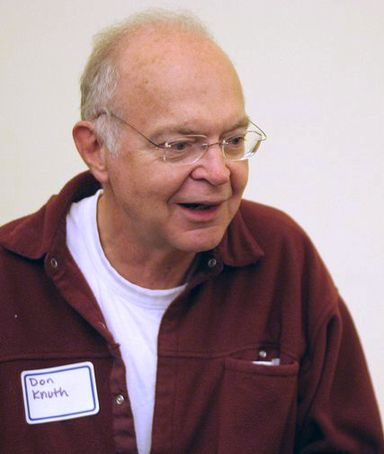
\includegraphics[scale=0.6]{images/Donald_Knuth.jpeg}
    \caption{克努斯博士,注:图片来源为克努斯博士的维基百科}
\end{figure}

由于克努斯博士此次在数学公式的排版上下足了功夫,就在他启动这项计划不久后,他收到了美国数
学协会 (American Mathematical Society, AMS) 的邀请,克努斯博士在此次邀请中汇报的内容
是“基于TeX排版,如何让计算机服务于数学”,这次汇报成功吸引了一大批数学家的目光。由于TeX
在数学公式排版方面的优秀表现,比如数学公式的自动间距调整,TeX后来摇身一变成为了书写数学
公式的“利器”。

为了提升TeX的开发质量,克努斯博士悬赏奖励任何能够在TeX中发现程序漏洞的人,也就是我们一般
认为的“找bug”。每一个bug的奖励金额从2.56美元(16进制的100美分)开始,以后每发现一个bug,
都会翻倍,直到327.68美元封顶。然而,克努斯博士从未因此而损失大笔金钱,因为TeX中的bug极
少,而真正发现bug的人在获得支票后往往因其纪念价值而不愿兑现。

随着时间的推移,TeX也派生出了很多优秀的软件,其中最著名的派生软件便是LaTeX。另外,美国
数学学会也发布了TeX版本的数学公式宏包,其中,以ams命名的宏包就有\emph{amsfonts}、
\emph{amsmath}、\emph{amssymb}等,这些宏包都可以在LaTeX上进行使用,在LaTeX上使用这
些宏包可以编辑出各种数学公式。

\begin{tcolorbox}[colback=red!5!white, colframe=red!50!black, title=参考资料]
    TeX的维基百科介绍: https://zh.wikipedia.org/wiki/TeX.
\end{tcolorbox}

\section{引领浪潮的\LaTeX }
\subsection{\LaTeX 的出现}
LaTeX是一款高质量的文档排版系统,LaTeX在读法上一般发作Lay-tek或者Lah-tek的音,而不
是大家普遍认为的Lay-teks。LaTeX的历史可以追溯到1984年,兰波特博士作为早期开发者在这一年
发布了LaTeX的最初版本。事实上,LaTeX完全是兰伯特博士的意外所得,他当年出于自己写书
的需要,在早先发布的文档排版系统TeX基础上新增了一些特定的宏包,为了便于自己日后可以重复
使用这些宏包,他将这些宏包进行规整,于是,便有了相应的标准宏包 (standard macro package)。
谁曾想,正是这些不经意间开发出来的宏包,在经过后续封装和发布使用手册之后,形成了LaTeX的
雏形。

\begin{figure}
    \centering
    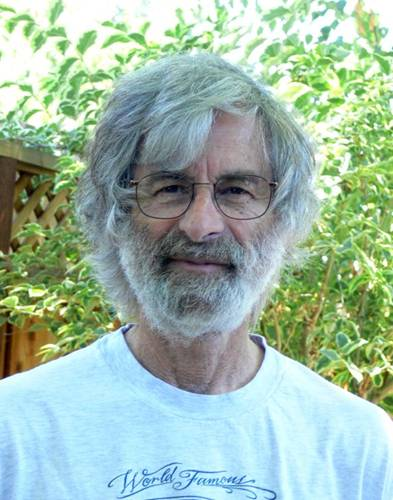
\includegraphics[scale=0.6]{images/Leslie_Lamport.jpeg}
    \caption{兰伯特博士,注:图片来源为兰伯特博士的维基百科}
\end{figure}

在很长一段时间里,LaTeX的版本其实没有多少大的更新,从技术层面来说,LaTeX实在没有什
么可供更新的地方了,它最初的面貌已趋近于完美且深入人心。LaTeX的最初版本是由兰伯特博士
于上世纪80年代初开发出来的,目前,广泛使用的版本LaTeX2e是在1994年发布的,发布后一直没有
大的更新,甚至发布后的首次更新出现在二十多年后的2020年。尽管LaTeX2e的后续版本更新工作早
在上世纪九十年代初就已经开展了,但时至今日,新版的LaTeX仍未进入人们的视野。从开发者兰伯
特博士的角度来看,开发LaTeX的目的是为了降低TeX的使用门槛、更容易地发挥TeX强大的排版功能,
提供一款高质量、解释性强的计算机程序语言,所以LaTeX最初的风格就是精简,这也是为什么LaTeX
在日后可供提升的地方不是很多的原因。

\subsection{\LaTeX 的特点}
由于种种原因,时至今日,TeX几乎淡出了人们的视线,不过我们现在依旧能看到:在使用LaTeX制作
文档时,通常需要创建一个以\emph{.tex}为拓展名的文件。对于很多人来说,日常制作各类文档的
首选可能是Word等软件,它简单好用、所写即所见,但当我们制作几十页甚至上百页的文档时,Word
的劣势就会展露无疑,因为我们需要投入大量的时间和精力来对文档内容进行排版。反观LaTeX,它
对文档的排版都是自动完成的,我们根本不需要像Word那样完全手动调整格式,另外,使用LaTeX插
入各种图形、表格、公式、文献时,相应的索引出错的可能性也非常小,这些优点都是Word所无法
比拟的。

在上个世纪80年代和90年代,LaTeX的用户群体非常庞大,然而,在世纪之交,随着微软推出的一系
列Windows操作系统快速发展,例如红极一时的XP系统,相应的办公软件Microsoft Office也以其
便捷性吸引了人们的视线,致使大量LaTeX用户转而使用Microsoft Office。即便如此,时至今日,
LaTeX的用户群体依旧十分庞大,这主要得益于LaTeX强大的文档排版能力,虽然LaTeX复杂的语法结
构、不容配置的编译环境让很多初学者望而却步,但LaTeX能让用户更专注于内容创作,而非锦上添
花的“排版”,这一显著特点契合了人们对质量和效率的追求,使得LaTeX在文档排版、论文撰写等方
面占有重要地位。在此基础上,具体来说,使得LaTeX历久弥新的关键可以归纳为以下五点:
\begin{enumerate}
    \item LaTeX是专门用于制作文档的计算机程序语言。在众多计算机程序语言中,LaTeX可以制
          作排版连贯性极好的专业文档。
    \item 独特的创作方式。尽管LaTeX沿用了TeX排版系统,但使用LaTeX制作文档时,内容创作
          和文档生成却是分开的,有需要的时候,我们可以预览创作的文档。因此,在创作的过程中,
          创作者不再像使用办公软件Word那样,既要关注创作内容,又要同步关注繁琐的排版和格式,
          使用LaTeX制作文档能在真正意义上让创作者专注于创作内容本身。更值得一提的是,当文档篇
          幅较大时,使用LaTeX无疑会让我们节省大量的时间和精力。
    \item 简单的逻辑结构。使用LaTeX制作文档时,创作者可以通过一些非常简单的逻辑结构进行
          创作,如chapter(章)、section(节)、table(表格)。因此,LaTeX的使用门槛并不像
          真正的程序语言那么高。很多人或许在使用LaTeX的过程中都不会用到for等基本的循环语句。
    \item 对数学公式以及特殊符号的支持程度。众所周知,LaTeX在开发之初,是作为数学和计算
          机相关研究人员的创作工具,这类群体喜欢使用LaTeX的原因无外乎是LaTeX可以通过一些简单
          的代码生成复杂的数学表达式和特殊符号。
    \item 编译以\emph{.tex}为拓展名的LaTeX文件后会得到一个PDF文档,PDF文档不存在跨
          平台、兼容性等问题,可以在各种操作系统上打开。
\end{enumerate}

当然,除了上述五点,实际上可能还有十分重要的一点,那就是LaTeX能够制作各类文档,从科技
论文、技术报告、著作、学位论文、幻灯片甚至到科技绘图一应俱全,当然它也支持嵌入图片、绘制
图形、设计表格、插入参考文献等。

从LaTeX的出现到当下,它已经形成了一套非常高效的文档制作环境:
\begin{itemize}
    \item 文档类型 (document class)。文档类型是文档排版样式的基调,这些类型包括
          文章 (article)、报告 (report)、幻灯片 (beamer)等,在.tex文件中申明文档类型后,
          我们就可以开始文档创作了。
    \item 宏包 (package)。它是LaTeX中的重要辅助工具,也可以把它理解为一般意义上的工具
          包。在使用时,调用宏包的基本命令为\emph{\textbackslash usepackage{}},举例来说,包含颜色命令的
          宏包为\emph{color},其调用语句为\emph{\textbackslash usepackage{color}}。随着LaTeX的发展,越来
          越多的宏包被开发出来,这些宏包能满足特定的需求(如制表、插图、绘图),同时也能让
          LaTeX代码变得更加简洁,我们只需要用简单的\emph{\textbackslash usepackage{}}命令就能调用
          所我们需要用到的宏包。
    \item 模板 (template)。LaTeX的发展催生了很多视觉和审美效果极好的模板,包括论文模板、
          幻灯片模板、报告模板甚至著作模板,这些模板在一定程度上能减少创作者在文档排版上的时间
          开销,也有很多学术刊物会给投稿作者提供相应的LaTeX模板。
\end{itemize}

通过对比LaTeX和Word,我们还会看到:
\begin{itemize}
    \item 第一,LaTeX的.tex源文件是无格式的,编译之后,根据特定的模板和指定的格式形成
          最终的PDF文档,因此,使用LaTeX制作各类文档能够很方便地切换模板和修改格式;
    \item 第二,LaTeX对公式、图表以及文献引用的支持是Word所无法比拟的,尤为特殊的是,
          当文献数量达到上百篇时,在Word中修改参考文献可能是“牵一发而动全身”,费时耗力,而
          LaTeX根据已经整理好的\emph{.bib}文件可自动完成文献引用和生成。
\end{itemize}

\subsection{\LaTeX 编辑器}
实际上,配置LaTeX环境包括两部分,即编译器和编辑器,对应的英文表达分别是editor和complier,
两者不是一回事。LaTeX编译器又称为LaTeX编译工具,可根据系统安装相应的编译工具:
\begin{itemize}
    \item Linux系统:可安装TeX Live,该编辑器拥有LaTeX编辑器;
    \item Mac OS系统:可安装Mac TeX,该编译器拥有完整的TeX/LaTeX环境和LaTeX编辑器;
    \item Windows系统:可安装MiKTeX或TeX Live,两者都拥有完整的TeX/LaTeX环境和LaTeX编辑器。
\end{itemize}

目前,我们可以接触到很多LaTeX编辑器,这些编辑器的界面大致有两部分组成,即LaTeX源码编译
区域和PDF文档预览区域。前面也提到了几款LaTeX编译器,但如果想要提高LaTeX的使用体验,以下
几款LaTeX编辑器比较受人推崇:
\begin{itemize}
    \item TeXworks:这是TeX Live自带的一款轻量级编辑器。
    \item TeXstudio:这款编辑器集代码编译与文档预览于一身。
    \item WinEdt:这是CTeX自带的一款编辑器。
    \item VS Code:这是微软推出的一款免费文本编辑器,功能包括文本编辑、日常开发等。
    \item Atom:这是一款开源的跨平台编辑器(GitHub网址为https://github.com/atom/atom),
          支持多种程序语言。
\end{itemize}

\section{应运而生的在线系统}
\subsection{\LaTeX 在线系统的出现}
上世纪80年代,LaTeX作为一件新生事物,在发布之初便引起了人们极大的兴趣,虽然在制作文档方
面拥有很多办公软件都无法比拟的强大优势,尤其在数学公式编写及高效排版上具有很大优势,但是
由于其较高的使用门槛(使用计算机程序语言进行编译)和安装成本(本地安装需要花费大量的时间
配置相应的环境),在很长一段时间里,LaTeX主要用户都是科研工作者。然而,LaTeX在线系统的
出现已实实在在地改变了这一尴尬局面。

随着信息技术快速发展、互联网深度普及,人们的工作生活方式也在发生着很大改变,很多过去安装
在本地的操作软件都被搬到了浏览器上,人们无须在个人计算机上安装各类办公软件就能进行办公,
这带来了极大的便利。不过这类在线系统也存在一些先决条件,例如,出于计算资源方面的考虑,通
常要求在线系统的类型不能是计算密集型,因为计算密集型的在线系统往往需要大量的计算资源作支
撑。反观LaTeX,尽管我们可以认为LaTeX是一种计算机程序语言,但实际上,其对计算资源的需求
并不是很大。

在过去,受网速限制,使用线上系统几乎是一件难以想象的事。然而,在线系统的兴起并非空穴来风,
一方面是目前的网速已经跟过去发生了质的变化,另一方面则是上网成本在急剧降低,互联网触手可
及,已经成为人们日常生活和工作中不可或缺的一部分。以前,我们可能已经习惯了在本地计算机上
安装和使用各类软件或者集成开发环境,不过以LaTeX为例,在本地计算机上安装的集成开发环境也
有很多缺陷:
\begin{itemize}
    \item 第一,我们需要为安装LaTeX编辑器腾出很大的存储空间;
    \item 第二,某些特定的宏包需要额外安装和配置,但安装过多宏包之后又会使LaTeX变得很臃肿,
          甚至是不友好;
    \item 第三,当我们在本地计算机使用LaTeX制作文档时,我们很难与合作者进行协同创作。
\end{itemize}

在这个背景下,一些成熟的LaTeX在线系统逐渐走进人们的视野,并受到很多用户的喜爱,其中,最
为著名的LaTeX在线系统便是\emph{overleaf.com}。这些LaTeX在线系统不仅支持各种语言、各种
拓展宏包等复杂的LaTeX环境,同时也支持实时编译和实时预览编译后的文档,就算是换一台电脑,
也丝毫不会影响创作过程,创作完成之后,可以选择下载压缩文件包(如.zip),也可以只导出PDF
文档,毫无疑问,这些人性化的设计都是为了让LaTeX更加便捷和高效。除此之外,现有的LaTeX在
线系统还提供大量的LaTeX模板库,科技论文、毕业设计、幻灯片、海报、简历等参考模板一应俱全,
就连LaTeX使用文档也数不胜数。

\begin{tcolorbox}[colback=red!5!white, colframe=red!50!black, title=在线系统 overleaf]
    Overleaf是一个初创的科技企业,它的主要业务是构建现代化协作创作工具,即LaTeX在线系统,
    旨在让科学研究变得更加便捷和高效。
    目前,Overleaf已合并另一款著名的LaTeX在线系统ShareLaTeX,在全球范围内拥有超过600万
    用户,这些用户大多是来自于高校和研究机构的研究人员、老师以及学生,只要打开网址overleaf.com,
    用户无需在本地计算机配置LaTeX环境就可以创建各种LaTeX项目。
    \tcblower
    关于Overleaf的介绍可参考https://www.overleaf.com/about。
\end{tcolorbox}

\begin{figure}
    \centering
    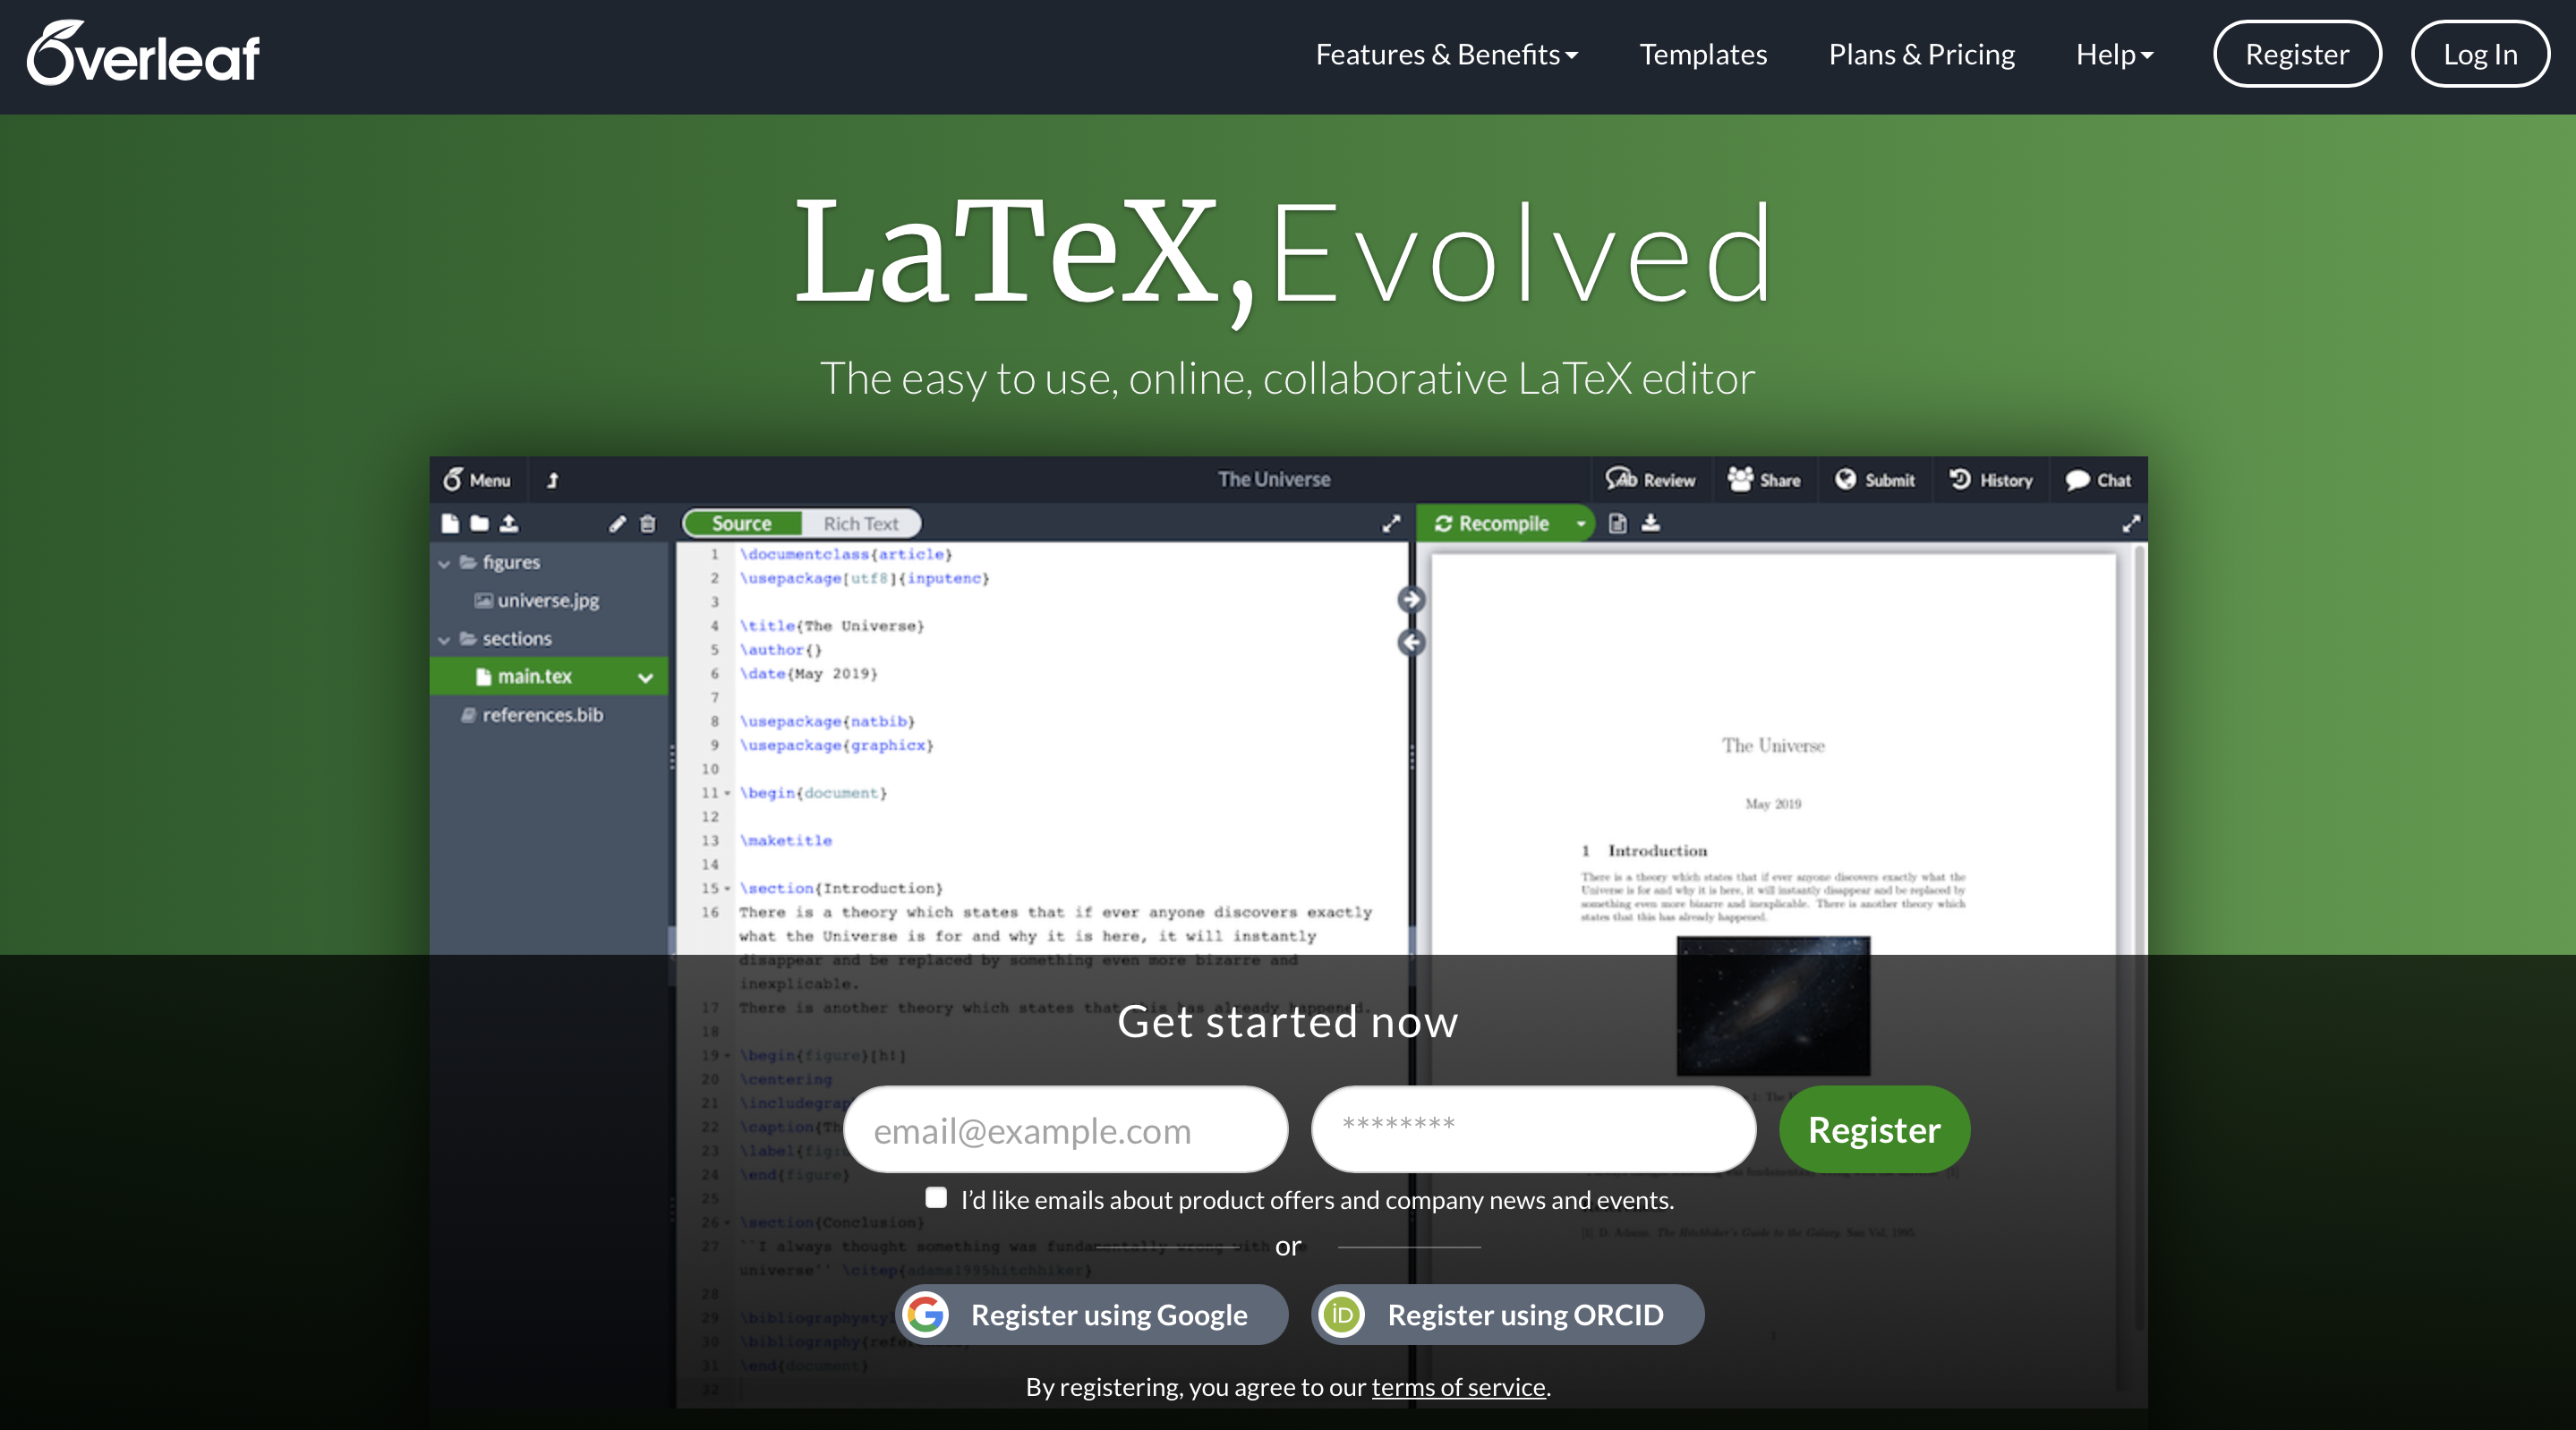
\includegraphics[width=\textwidth]{images/overleaf_webpage.png}
    \caption{Overleaf首页,图片来源于Overleaf官网}
\end{figure}

\subsection{\LaTeX 在线系统的特点}
以Overleaf为例,该LaTeX在线系统往往具备以下几点特征:
\begin{itemize}
    \item 免费和开源。可以免费注册和使用,不用下载和安装LaTeX编辑器,这一点对于初学者
          来说无疑是非常友好的;
    \item 使用简单。不管是在计算机、手机还是其他终端上,我们只需要使用浏览器打开overleaf.com
          就可以开始创作,另外,由于Overleaf界面非常简洁,所以用户使用起来也非常便利;
    \item 支持实时在线编辑。有各类LaTeX插件,编辑功能十分完善,且具有实时编译和预览功能;
    \item 支持在线协作。创作文档时,我们可以将文档项目分享给合作者进行协作,Overleaf支持实时编译,
          不会出现版本控制混乱等问题;
    \item 支持双向定位。可以在LaTeX代码与PDF文档内容之间进行双向定位;
    \item 提供丰富的模板库。Overleaf有着非常庞大的模板库,不仅有正式的学术论文、学位论文
          和书籍的参考模板,还有很多美观的报告、简历、幻灯片模板。就论文写作来说,用户可以在Overleaf
          官网找到众多期刊的LaTeX模板,根据使用说明,用户很容易就能用于撰写自己的论文;
    \item 提供大量的帮助文档。LaTeX提供了齐全的帮助文档,从LaTeX快速入门、基础操作到编译
          数学公式,应有尽有、一应俱全,且这些文档内容具有很强的实操性。
\end{itemize}

\begin{figure}
    \centering
    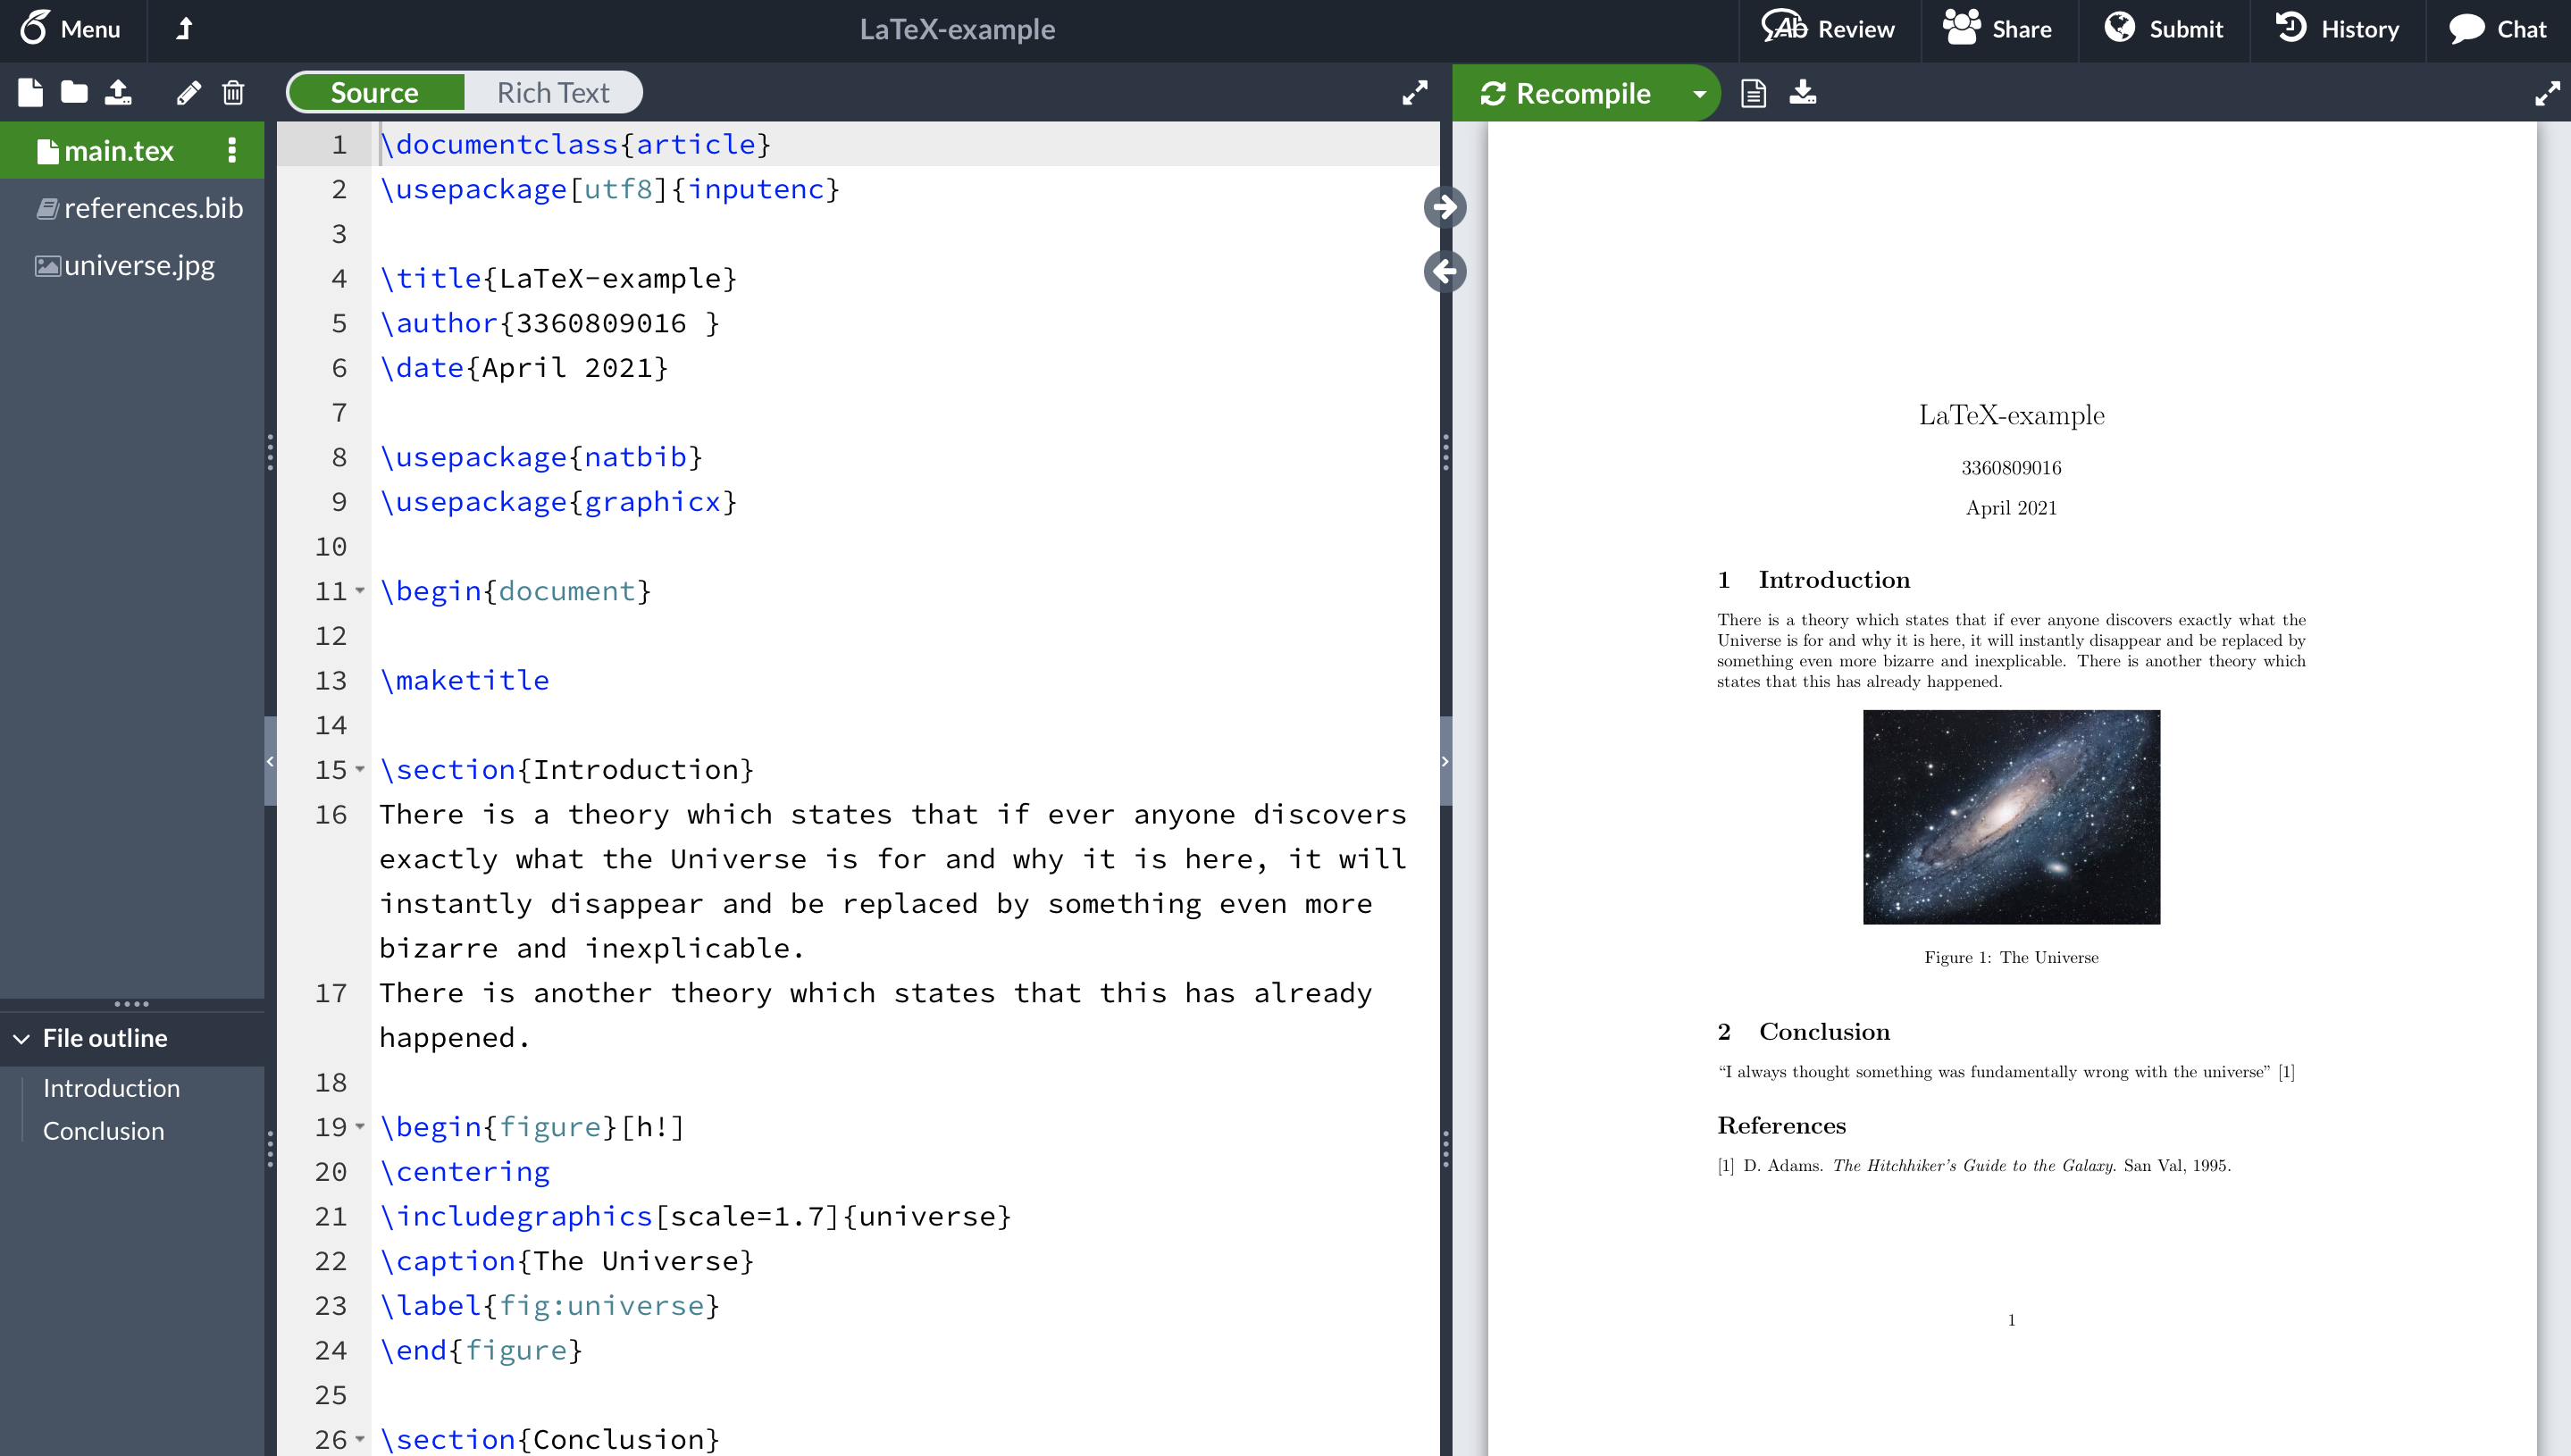
\includegraphics[width=\textwidth]{images/overleaf_example.png}
    \caption{Overleaf编辑器界面,主要由代码区域和文档预览区域组成}
\end{figure}

LaTeX在线系统的出现大大降低了LaTeX的使用门槛,也为用户省去了繁琐的安装和配置过程。其实,
LaTeX在线系统的出现并非个例,很多办公软件为迎合用户需求和时代发展趋势,陆续转变了产品研
发思路,包括微软在线Office系统、腾讯在线文档等在内的很多在线系统都走进了人们的视野,这些
在线系统能够在线备份、满足人们对随时随地办公的需求,在确保便捷和高效的同时,在线和共享的
理念正在潜移默化地影响着人们的办公模式。

\section{\LaTeX 问答社区}
在LaTeX刚被发布和推出的那个年代,相关资源如使用手册、教程等远没有今天这么丰富,同时,获
取渠道也没有今天这么便捷。在互联网触手可及的今天,我们能通过一个浏览器访问到各种相关学习
素材,遇到代码bug,也能在一些专业的问答社区找到最佳的解决方案。毫无疑问,对于今天的我们
来说,如何利用好互联网资源至关重要。

\subsection{问答社区的介绍}
对于从事计算机相关的技术人员来说,专业的技术问答社区往往是不可多得的资源,它能帮助很多技
术人员提升个人编程能力、学习新技术,同时解决一些技术困扰,例如解决编程时遇到的bug。对于
各类计算机程序语言而言,\emph{Stack Exchange}作为一个著名的技术问答社区,覆盖了大量编
程相关的技术问题和优质回答,就算是一些较为细致的问题,我们往往都能找到想要的答案。
Stack Exchange问答社区按计算机程序语言类型进行划分,我们所关心的LaTeX问答通常被分配在
TeX Stack Exchange社区(网址为https://tex.stackexchange.com/)。截至目前,
TeX Stack Exchange已经覆盖了关于TeX、LaTeX以及其他排版系统的用户在使用中遇到的诸多问题,
并且这些问题多与LaTeX相关。

\begin{tcolorbox}[colback=red!5!white, colframe=red!50!black, title=Stack Exchange]
    网址为https://stackexchange.com/,它与Stack Overflow问答社区在全球范围内拥有广泛的用户群体
\end{tcolorbox}

除了Stack Exchange这种涵盖了多种计算机程序语言的技术问答社区,LaTeX forum社
区(https://latex.org/forum/)是一个专门面向LaTeX的技术交流平台,它拥有非常活跃的用户
群体和丰富的问答资源,并拥有超过10万篇分门别类的技术帖子,我们可以根据浏览量从该平台一
览高频访问问题。

实际上,不管是LaTeX初学者还是高级用户,在遇到LaTeX使用问题时,去问答社区寻找解决方案都
是一种非常有效的方式。TeX Stack Exchange社区非常活跃,每天都会有大量关于LaTeX的问题和
回答,且每个问题下面的回答都会根据用户的认可度进行排序,回答一般比较细致。

\subsection{高频访问问题}
顾名思义,高频访问问题是指访问量较高的问题。LaTeX forum社区已经将众多问答帖子进行了分门
别类整理,针对某一特定话题,展开内容即可看到各类问题的访问情况。
